\section{Theory}
\label{sec:theory}
The aim of this experiment is to record the absoption spectrum
of rubidium. Therefore a diode laser is adjusted and aimed towards a cell
filled with rubidum.
The following sections introduce the theory
important for the understanding of the experiment.

\subsection{Laser basics}
\label{subsec:Laser}
A Laser (Light Amplification by Stimulated Emission of radiation)
emits highly intensive light with a long coherece length.
Fist of all the interaction of a radiation field with
a energy level system is considered. These includes
absoption and spontaneous and stimulated emission
of a photon, shown in figure \ref{fig:ab_em}.
\begin{figure}
\centering
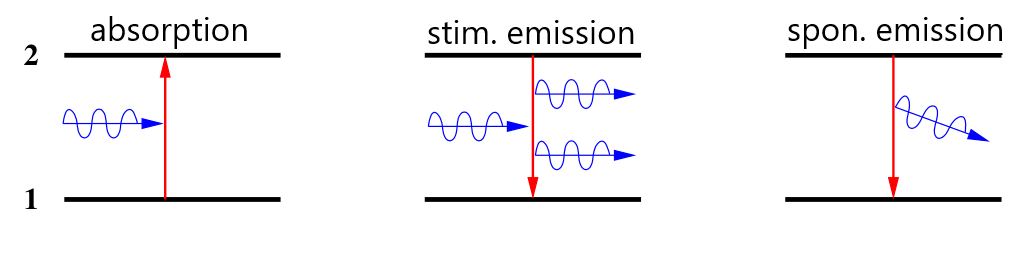
\includegraphics[width=0.7\textwidth]{ab_und_emiss.png}
\caption{Absorption and both spontaneous and stimulated emission of a photon in a two energy level system.
\cite{V61}}
\label{fig:ab_em}
\end{figure}
Absorption descripts the process where a photon annihilates and
delivers energy for the transition
to a higher energy level.
Spontaneous emission discripts the opposite, a photon is
emitted if a transition to a lower energy
level occurs spontaneously.
But most important for a laser as the name indicates
is the stimulated emission.
The process of stimulated emission works as follows.
If a photon with the energie same as
the energy gap between the two energy levels
encounters an excited state, an other photon with
same energy and phase is emmitted and the excited state
returns to the ground state.
To run a laser stimulated emission must be the commonest interaction.
Because of the occupation of the energy levels for fermion follows
the Fermi-Dirac statistics, % vielleicht doch hier noch von bolzmannstatistik sprechen
levels above the Fermi energy are
less occupied. By increases the temperature only
a same occupation can be accomplish.
However, this is not enough in order to ensure mostly stimulated emission.
Therefore a population inversion
between ground state and an excited
state is necessary. As to achieve this at least
a three level system is of need.
Transitions between the levels can be radiative as explained above
aswell as non radative for example in the form of lattice vibration.
Further the energy levels vary with regard
to the decay rate. In figure \ref{fig:3_n} the process of pumping and stimulated emission
is displayed for a three energy level system.
\begin{figure}
  \centering
  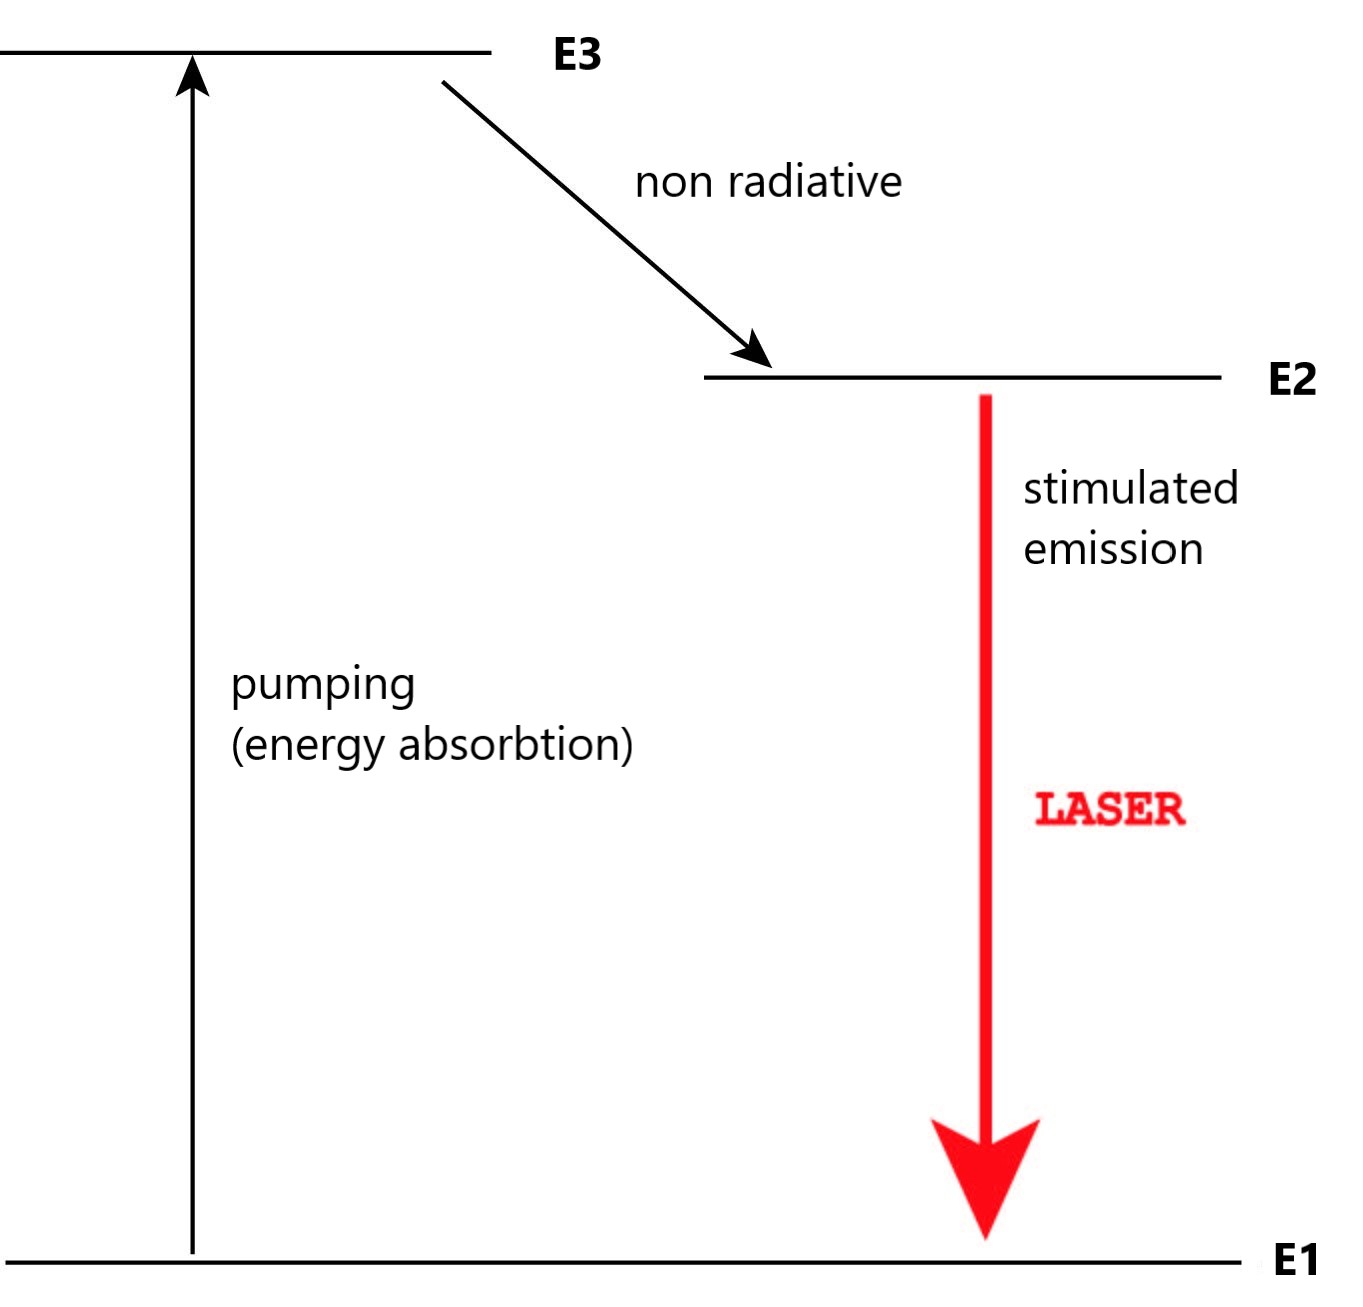
\includegraphics{Laser_3_Niveau.jpg}
  \caption{three energy level system}
  \label{fig:3_n}
\end{figure}
The Laser process for a three energy level system
goes as follows
The transition from \textbf{E1} to \textbf{E3} is induced
by absoption of energy.
The level \textbf{E3} have a high
decay rate form \textbf{E3} to \textbf{E2}
so a transition happens almost instantaneous
through nonradiative spontaneous emission.
Level \textbf{E2} compared to \textbf{E3}
has a lower decay rate.
So when energy is continuous
pumped into level \textbf{E1},
the required population inversion
between the groud state \textbf{E1} and the
excited state \textbf{E2} is created.
Now a photon which spontaneous is emitted
through the radiative decay from
\textbf{E2} to \textbf{E1}
leads to
stimulated emissions of other photons,
thus a highly intensive
light with a long coherece length.

Beside the theoretical approach to
accomplish laser radiation, some other criteria
must be also met.
First of all a gain medium with the desired
energy gab is necessary in which
a population inversion by pumping is created.
Pumping energy is supplied by light or electric current.
In addition the gain medium is bounded to a heat-sink
to dissipate residual heat, which is produced by pumping.
Further more a Laser cavity is required.
The Laser cavity consists of the gain medium and two
mirrors, one higly reflective and the other
partially transparent,
the output coupler.
In the figure \ref{fig:laserschema}
a schematic laser with its components is displayed.
\begin{figure}
\centering
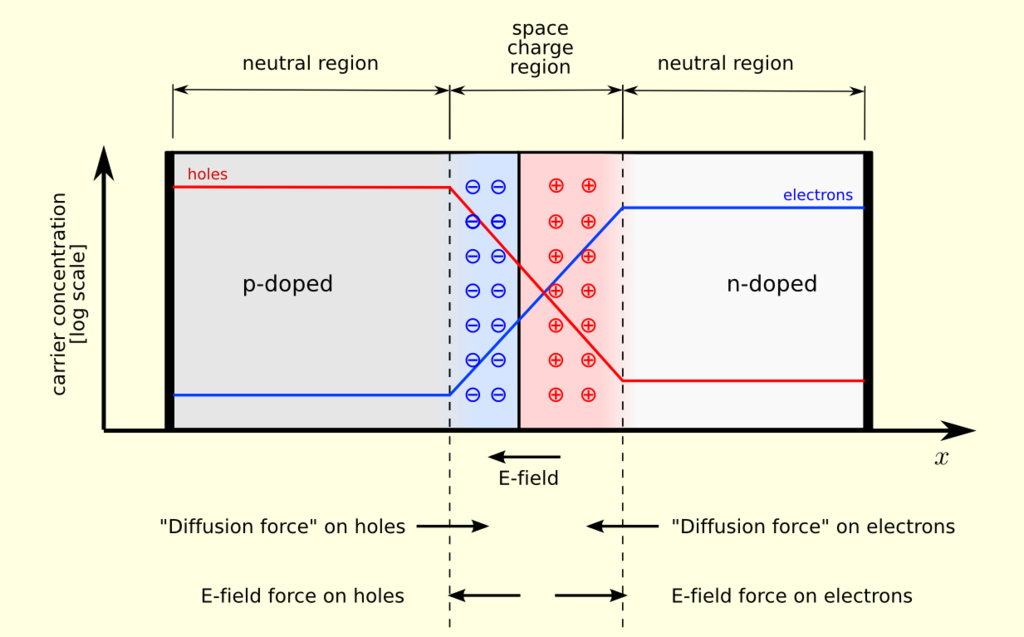
\includegraphics[width=0.7\textwidth]{equilibrium.png}
\caption{A schematic Laser and its components.
\cite{wiki_diode}}
\label{fig:equi}
\end{figure}
The operation of the Laser cavity is as followed.
Photons are emitted through spontaneous emission
in the gain medium. The two mirrows
ensure that the photons stay in the Laser cavity
and the Laser intenensity increases due to
stimulated emission of other photons.
Depeneding on the cavity lenght $L$
standing waves along the cavity axis so called longituidinal modes
are developed.
The modes vary according to the wavelength and hence
the the number of knots. The spacing
between frequencies of two modes in a laser
cavity is given by the free spectral range (FSR)
\begin{align}
\Delta \nu_{FSR} = \frac{c}{2Ln}
\end{align}
where $c$ is the speed of light and $n$ is
the index of refraction.
A development of transversal modes in the laser cavity
is also possible but is not discussed on detail further.
The laser ray that comes out of the output coupler
contains all the frequencies of the longituidinal modes.

\subsection{Semiconductor}
\label{subsec:Semiconductor}

The diode laser is a result of the reseaching done on semiconductor.
So first a deeper comprehension of semiconductor theory is needed.
Hence the principle funcion of a simple p-n diode is described.
A p-n diode exist out of two semiconductor materials one
n-type and the other p-type.
In the p-type semiconductor is an excess of holes
and in the n-type semiconductor, an exess of electrons.
An excess of holes or electrons can be accomplish by doping.
When n- and p-type are merged together,
electrons and holes diffuse in opposite side and recombine.
This process induce a elctricfield bettween the fixed doping atoms, which
counteracts the diffusion process.
If equilibrium between the two forces is accomplish
a charge depletion zone is created
at the p-n junction.
The figure \ref{fig:equi} shows
a schematic p-n Diode in equilibrium.

\begin{figure}
\centering
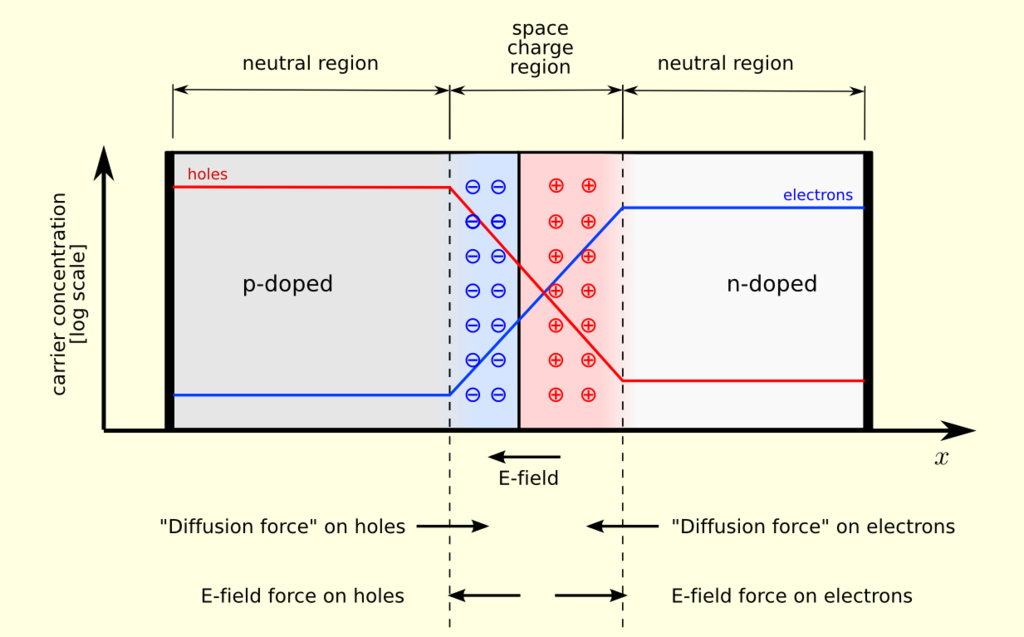
\includegraphics[width=0.7\textwidth]{equilibrium.png}
\caption{A schematic p-n Diode in equilibrium.
\cite{wiki_diode}}
\label{fig:equi}
\end{figure}

There are two possible ways apply voltage
in forward bias and
in rewerse bias.
In forward bias the diode let the curruent follow
but in the rewese bias the diode bocks the current up to the breaking point.
A typical diode characteristic is shown in figure \ref{chara}
\begin{figure}
\centering
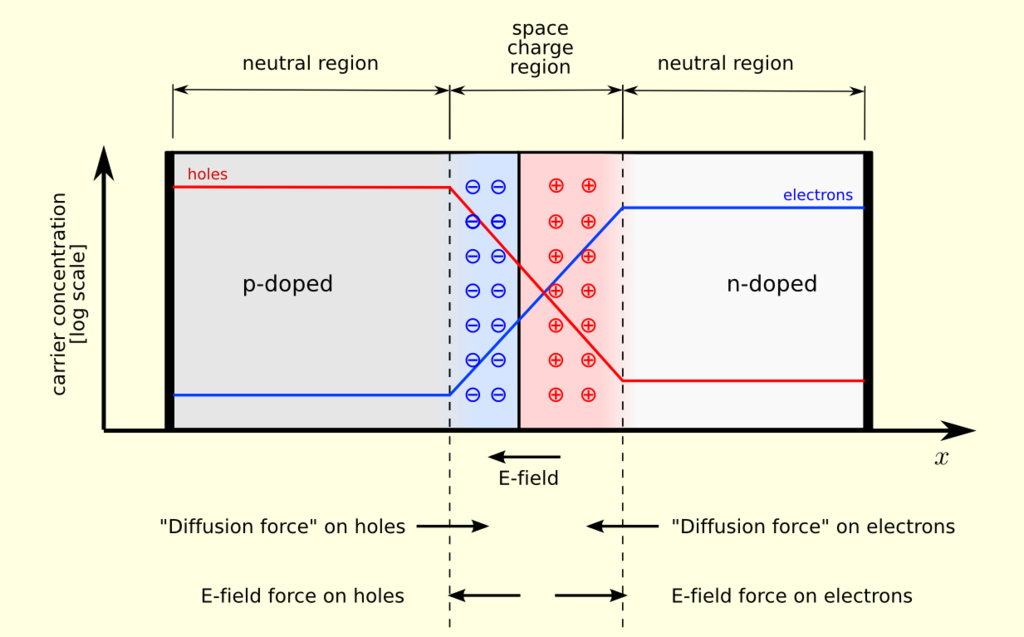
\includegraphics[width=0.7\textwidth]{equilibrium.png}
\caption{A schematic p-n Diode in equilibrium.
\cite{sparkfun}} % https://learn.sparkfun.com/tutorials/diodes/real-diode-characteristics
\label{fig:chara}
\end{figure}
For the Diode Laser a light-emitting diode (LED)
is necessary. A LED differ in terms of
the band gab
from a simple p-n diode.
For a LED a direct band gab is needed, so a photon
with the energy of the band gab is
emitted if electrons and holes recombine.

\subsection{Diodenlaser}
\label{sec:Diodenlaser}
By applying the informations of previous sections
a diode laser can be explained.
The diode laser consist of a special semiconductor chip.
The chip has a certain structur shown in figure \ref{fig:chip}.
\begin{figure}
  \centering
  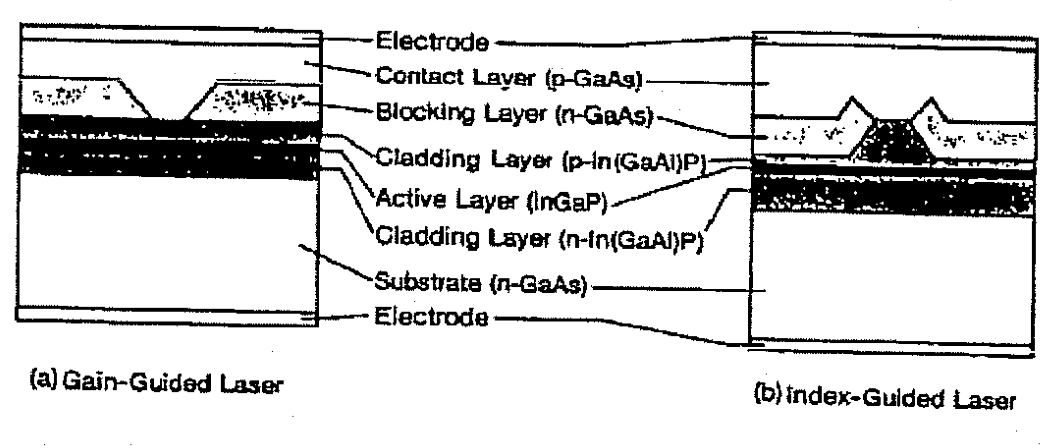
\includegraphics[width=0.7\textwidth]{chip.png}
  \caption{Two different typical structurs profiles of a diode laser chip.}
  \label{fig:chip}
\end{figure}
The active layer of the chip has a higer refraction index than
its surroundings. Because of that light which is emmitted
in the active layer through recombination of electron-hole pairs
is confined in the channel by total internal reflection.
The cleaved facets at the end of the chip
are coated to incraese or decrease the facet reflectivity
The cavity mirrors and output couplers arise
by coating the cleaved facets at the end of the chip,
to increase or decrease the facet reflectivity.
So a tiny semiconductor laser cavity inside the chip
with a typical linewidht
$\delta \nu \approx \SI{50}{\mega\hertz}$
is developed.
A population inversion
can be achieved through current.
But at low levels of current
the optical losses are higer than the gain
so a population inversion is not achieved and
the laser diode emits a broad-band light
through spontaneous emission
like a LED.
To obtain a coherent laser beam the current must be above
a threshold current where the gain is higher than the
optical losses so a population inversion is created.
Futhermore the laser intensity increases linearly with
injection current.
The output beam of chip is elliptical an strongly diverging
therefore a collimating lens is necessary.
Still there are two Problems to solve.
First the diode laser is very sensitive to optical feedback
already $10^{-6}$ of the output light affects
the stability of the frequence
when scattered back in the
laser cavity.
Therefore a diffraction grating is installed which
is shown in figure \ref{fig:aufbau}.
\begin{figure}
  \centering
  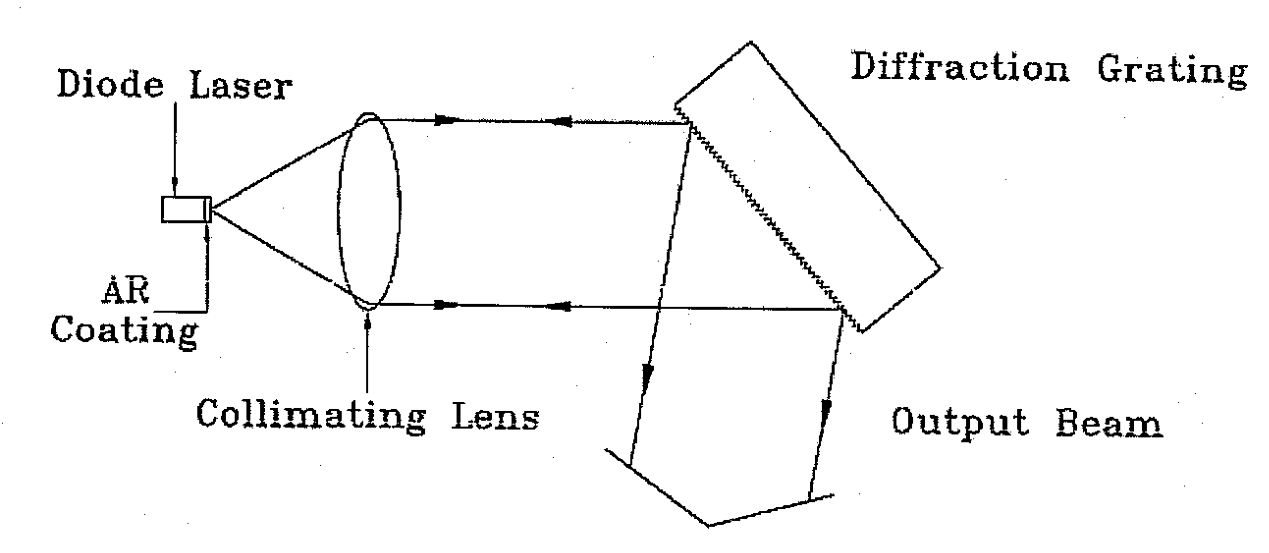
\includegraphics[width=0.7\textwidth]{aufbau.png}
  \caption{Schematical layout of a diode laser with collimating lens and diffraction grating.}
  \label{fig:aufbau}
\end{figure}
The diffraction grating ensure that

The diffraction grating fortunately solves the second
problem which is the large linewidth of the bare
diode laser($\delta \nu \approx \SI{50}{\mega\hertz}$)
compared to the linewidth of atomic transitions
(here $\Gamma \approx \SI{5}{\mega\hertz}$).
The grating and the


\subsection{Diodenlaser}
\label{subsec:diodenlaser}


\subsection{Beiträge im Laser}
\label{subsec:}



\subsection{Rubidum spektrum}
\label{subsec:}


\subsection{piezo}
\label{subsec:}
